\pagelayout{wide} % No margins
\addpart{\Nb nuclear spin}
\pagelayout{margin} % Restore margins
\setchapterpreamble[u]{\margintoc}

\chapter{Precision spectroscopy of a \Nb nuclear spin}
\label{ch:nb_nuclear_spin}

\begin{quote}
\itshape
In this chapter we investigate an unexpected nuclear spin found in close-proximity to an individual \Er spin. We initially identify the spin through spectroscopy of the electron spin transitions, of which there are ten, indicating that the nuclear spin has $I=9/2$. By analysis of the NMR transitions, excited through stimulated Raman driving, we identify the spin as a \Nb. 

We proceed to perform precision spectroscopy by leveraging the long coherence of the \Nb spin, and we are able to determine the nuclear transition frequencies with a Hz precision. By fitting the nuclear spectra to a Hamiltonian model we identify a previously unobserved form of electrical coupling between the electron and the nuclear spin as well as set a higher bound on the hexadecapolar interaction of the \Nb nuclear spin.
\end{quote} 

\section{Introduction}

Precision measurements of the hyperfine spectrum of atoms and simple molecules probe electron-nuclear interactions beyond the leading-order magnetic dipolar and electric quadrupolar terms~\sidecite{schwartz_theory_1955}. Higher-order interactions such as the magnetic octuple are $\sim 10^5$ times weaker; hence, high spectral resolution ($\sim $Hz) is required to resolve their contribution. This is readily achieved in atomic and molecular beams or in single-ion experiments, using combined microwave and laser excitations~\sidecite{gerginov_observation_2003,lewty_spectroscopy_2012}. In the solid state, ensemble magnetic resonance measurements of coupled electron-nuclear spin systems generally offer a lower spectral resolution (kHz at best~\sidecite{sielaff_pulsed_2025}), particularly when high-spin nuclei are involved. Indeed, the lines are broadened due to a combination of spin-spin interactions and inhomogeneous distribution of electron gyromagnetic tensor and/or quadrupolar couplings. This precluded so far the observation of higher-order terms in the coupled spin Hamiltonian by magnetic resonance techniques, despite active research~\sidecite{segel_nuclear_1978,doering_search_1986,liao_nuclear_1994}.

Major progress in spectral resolution was brought by recent experiments carried on individual paramagnetic centers in ultra-pure crystals at low temperature, opening the way to precision hyperfine spectroscopy in the solid-sate. The hyperfine and quadrupolar interactions of $^{13}\mathrm{C}$ and $^{14}\mathrm{N}$ nuclear spins in diamond were measured with Hertz resolution by a Nitrogen-Vacancy (NV) center spin, using optical detection of the NV at 4K~\sidecite{abobeih_atomicscale_2019, vandestolpe_mapping_2024, bartling_universal_2025}. Hertz resolution was also reported for the spin Hamiltonian parameters of $^{31}\mathrm{P}$ and $^{123}\mathrm{Sb}$ nuclear spin ($I=7/2$) of an electron spin donor in $^{28}\mathrm{Si}$-enriched silicon, using spin-to-charge conversion of the donor at 10mK for detection~\sidecite{fernandezdefuentes_navigating_2024}. 

\section{Spin system}

\begin{figure*}[t!]
    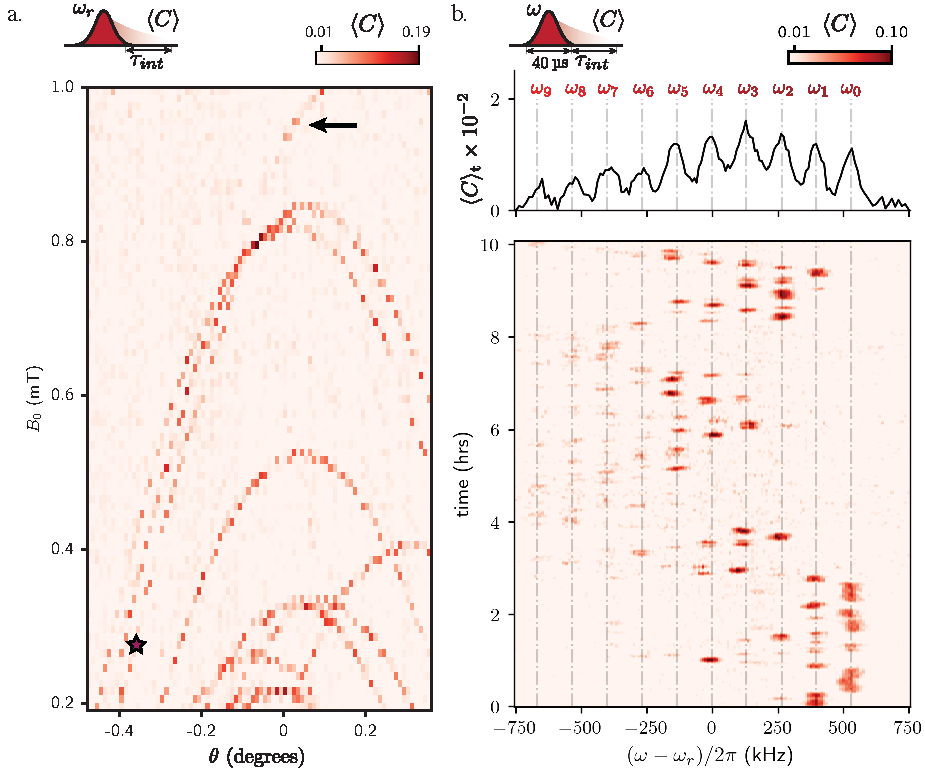
\includegraphics{chapter5/figures/spectra_2d.pdf}
    \caption[Rotation pattern and time trace of \Nb -- \Er system]{Rotation pattern and time trace of \Nb -- \Er system. \textbf{a.} Rotation pattern. The ensemble averaged counts $\langle C \rangle$ is plot as a function of the magnetic field amplitude and the angle $\theta$. The black arrow marks the \Er spin that is strongly coupled to the \Nb nuclear spin. The red star marks the magnetic field amplitude and $\theta$ used for this work.
    \textbf{b.} Spectroscopy of the \Er - \Nb coupled system as a function of time. A Gaussian pulse with duration 40 \textmu s and frequency $\omega/2\pi$ is first applied to the sample. After a waiting time $\tau_{\text{w}}=120$~\textmu s, photon counts from the SMPD are integrated over a window of length $\tau_{int}=2$~ms. The same pulse-and-readout sequence is then repeated at the next pulse frequency. The ensemble-averaged signal $\langle C \rangle$ is obtained by averaging 1000 integrated count values. The bottom plot shows the time averaged signal $\langle C\rangle _{\mathrm{total}}$  as a function of pulse frequency. Gray dashed lines have been plot as a guide for the eye for each EPR transition with frequencies $\omega_{n}$.}
    \labfig{spectra_2d}
\end{figure*}

As discussed in previous chapters, the sample hosts many addressable single \Er spins, each with its unique nuclear spin environment. The coupled \Nb -- \Er spin system was discovered fortuitously in the same \Ca sample used during the previous experiments. \reffig{spectra_2d}a shows a large range electron spin 2D-spectroscopy, where both the amplitude and the in-plane angle of the external magnetic field $B_0$ are swept. The spin of interest in this chapter is marked with a black arrow.

\begin{margintable}
    \centering
    \begin{tabular}{l|c}
    Parameter & Value \\ \hline
    $T_1$        & 0.47(2) ms  \\ 
    $g_0/2\pi$   & 9.3(0.1) kHz \\ 
    $T^*_2$      & 0.10(2) ms   \\ 
    $T_2$        & 0.35(1) ms  \\
    \end{tabular}
    \caption[\Er characterization]{\Er characterization.}
    \labtab{er_characterization_nb}
\end{margintable}

To characterize the \Er spin, we first set $B_0$ to match the ion resonance condition. Unless otherwise specified, the measurements of this chapter were taken at the point marked in \reffig{spectra_2d}a as a red star. The results of the basic electron spin characterization are detailed in \reftab{er_characterization_nb}.

We then measure a spectroscopic time trace\sidenote{Similar to the ones presented in \refsec{nuclear_spin_quantum_jumps}} repeatedly measuring the \Er resonance spectrum by sweeping the excitation pulse frequency and monitoring the subsequent fluorescence. Note, that the operating bandwidth of the SMPD is $\sim300$~kHz, much smaller than the span of the scan. To measure this trace we actively tune the frequency of the detector using DC pulses sent through the buffer's flux line, which modifies the magnetic flux threading the coupled SQUID, therefore changing the frequency of the SMPD. 

As shown in Chapter \ref{ch:detection_and_control_of_individual_w}, strongly coupled nuclear spins are revealed by sudden jumps of the \Er resonance, due to changes on the state of neighboring nuclear spins, strongly coupled to the \Er ion via hyperfine interaction. In \reffig{spectra_2d}b, ten evenly-spaced resonances are observed, they are separated by $\sim$130~kHz and have with vastly different cross-relaxation lifetimes, indicating the coupling to a spin-9/2 nuclear spin impurity.  

As discussed in \refsec{nb_er_hamiltonian} the Hamiltonian of such a coupled spin system is given by

\begin{equation}
    \cH{}/\hbar = \omega_S \hat{S}_z + \omega_I \hat{I}_z + A_\parallel \hat{S}_z \hat{I}_z + A_\perp \hat{S}_z \hat{I}_x + \hat{\mathbf{I}} \cdot \bar{\bar{Q}} \cdot \hat{\mathbf{I}}.
    \label{eq:hamiltonian_ninehalf_full}
\end{equation}

where the terms correspond, in order, to the \Er spin Zeeman energy, the high-nuclear spin Zeeman energy the parallel and perpendicular interaction hyperfine interaction and the quadrupolar term. This last term describes the nucleus electrostatic energy in the electric field gradient caused by the surrounding charges. The Hamiltonian can be re-written as

\begin{align}
\begin{split}
    \mathcal{H} = &\ket{\Downarrow}\bra{\Downarrow}\otimes \mathcal{H}^{(\Downarrow)} + \ket{\Uparrow}\bra{\Uparrow}\otimes \mathcal{H}^{(\Uparrow)} \\
    \mathcal{H}^{(\Downarrow)}/\hbar &= -\omega_S / 2 + \omega_I^{(\Downarrow)} I_z^{(\Downarrow)} + \mathbf{I}\cdot \bar{\bar{Q}}^{(\Downarrow)}\cdot \mathbf{I} \\ 
    \mathcal{H}^{(\Uparrow)}/\hbar &= +\omega_S / 2 + \omega_I^{(\Uparrow)}I_z^{(\Uparrow)} + \mathbf{I}\cdot \bar{\bar{Q}}^{(\Uparrow)} \cdot\mathbf{I}.
\end{split}
\label{eq:up_down_hamiltonian}
\end{align}


\noindent  $\mathcal{H}^{(m_S)}$ is the nuclear spin Hamiltonian when the \Er spin is in $m_S = \Downarrow$ or $m_S = \Uparrow$. As a result of the hyperfine interaction, the nuclear spin quantization axis $z^{(m_S)}$ and Larmor frequency $\omega_I^{(m_S)} \simeq \omega_I + m_S A_\parallel/2 $ depend on the \Er spin state. In the usual coupled spin description, the quadrupolar tensor should not depend on $m_S$. In this chapter we focus on testing this property by separately measuring the tensors $\bar{\bar{Q}}^{(\Downarrow)}$ and $\bar{\bar{Q}}^{(\Uparrow)}$ for each \Er spin orientation. 

\begin{marginfigure}
    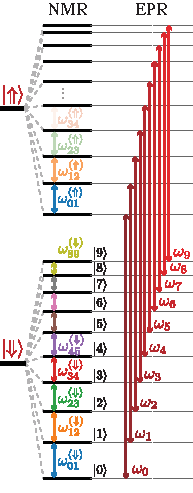
\includegraphics{chapter5/figures/energy_levels_ninehalf.pdf}
    \caption[Energy level diagram of an Er3+ coupled to a nuclear spin-9/2]{Energy level diagram of an Er3+ coupled to a \Nb nuclear spin-9/2. The twenty energy levels are separated in two manifolds, depending on the state of the electron spin. NMR-allowed and EPR-allowed transitions are represented as multi-colors and red arrows respectively.}
    \labfig{energy_levels_ninehalf_ch5}
\end{marginfigure}

We now recall the energy level system defined by this Hamiltonian. \reffig{energy_levels_ninehalf_ch5} shows the $20$ energy levels of the coupled spins, grouped in the two $m_S = \Downarrow$ or $m_S = \Uparrow$ manifolds. The nuclear spin eigenstates are mixed by the quadrupolar interaction and are therefore labeled as $\ket{n}$ in increasing order of energy, with $n$ varying between $0$ and $9$. Ten transitions between $\ket{\Downarrow, n}$ and $\ket{\Uparrow, n}$ at $\omega_n$ are EPR-allowed. Transitions between $\ket{m_S, n}$ and $\ket{m_S, n+1}$ at frequencies $\omega_{n,n+1}^{m_S} $ are NMR-allowed. Double- or Zero-quantum transitions between $\ket{\Downarrow, n}$ and $\ket{\Uparrow, n \pm 1}$ are weakly authorized because of the slight difference of nuclear spin wave function when the \Er spin is $\ket{\Downarrow}$ and $\ket{\Uparrow}$.


\section{Readout, preparation and control}

After the identification of the high-nuclear spin species we proceed to extend the nuclear spin single-shot readout, DNP and coherent control techniques developed in the previous chapters for the characterization of \W nuclear spins.

\subsubsection{Single-shot readout}

\begin{marginfigure}
    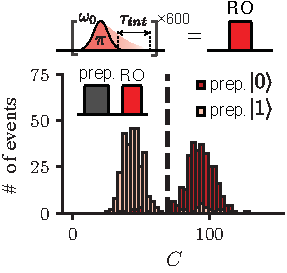
\includegraphics{chapter5/figures/readout_singleshot.pdf}
    \caption[Single-shot readout of the \Nb spin state]{Single-shot readout of the \Nb spin state. 
    \textit{(top)} Readout is defined as the application of 600 $\pi$-pulses with frequency $\omega_0$ and averaging the number of counts during an integration time $\tau_\text{int}=1$~ms after each pulse.
    \textit{(bottom)} Readout histograms after preparing the \Nb spin in $\ket{0}$ and $\ket{1}$, red and pink respectively. Inset shows the pulse sequence. A vertical dashed line marks the threshold used for state assignment.}
    \labfig{readout_singleshot}
\end{marginfigure}

During the experiments performed in Chapters \ref{ch:detection_and_control_of_individual_w} and \ref{ch:individual_nuclear_spins_quantum_information} with \W, the frequency separation between the electron spin transitions was in the order of $\sim50$~kHz, well within the SMPD and the resonator bandwidth. This allowed us to monitor the population of each of the nuclear spin states independently by exciting the appropriate electron spin transition and measuring the subsequent fluorescence (see \refsec{single_shot_ro_singlespin}). However, the ten distinct electron spin frequencies of this system are separated each by $\sim130$~kHz spanning more than 1~MHz, considerably larger than the SMPD and the resonator bandwidth. Additionally, the cross-relaxation probability of the different nuclear states is vastly difference, as evidenced by the different effective nuclear spin lifetimes in \reffig{spectra_2d}b. Consequently, we focus the nuclear spin readout protocol in the longest lived transition, the one with the highest frequency $\omega_0$. To maximize the Purcell effect in this transition we slightly tune the magnetic field such that $\omega_r = \omega_0$.

Readout on state $\ket{0}$ is achieved by applying $\sim 200$ successive $\pi$ pulses at $\omega_0$ and counting the number of clicks, $C$. Its distribution shows a well-resolved histogram, depending on whether the spin is prepared in $\ket{0}$ or in another state as shown in \reffig{readout_singleshot}. 

\subsubsection{Solid-effect polarization}

\begin{marginfigure}
    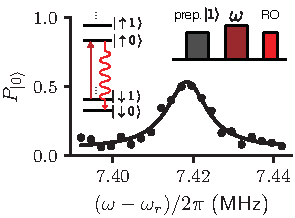
\includegraphics{chapter5/figures/zq_single_transition.pdf}
    \caption[ZQ transition spectroscopy]{Zero-quantum transition spectroscopy. $\ket{0}$ state population as a function of $\omega$ fit to a Lorentzian curve (solid line). The inset presents the energy diagram, where the straight arrow is the pumping pulse and the wavy line shows the most likely decay path.\red{replace to ZQ}}
    \labfig{zq_single_transition}
\end{marginfigure}

In the previous chapters we demonstrated how to perform solid-effect DNP to deterministically prepare the state of strongly coupled \W nuclear spins. The generalization to a high-nuclear spin $I=9/2$ is straightforward, as it only requires pumping all the $9$ DQ transitions to prepare $\ket{0}$. A crude approach would be to send a chirped pulse that covers a large frequency band of $10$~MHz under the electron spin transitions, this pulse would eventually excite one of the DQ transitions, bringing the nuclear spin state closer to $\ket{0}$. However, this technique is not time-efficient, as it chirps the pulse is mostly not resonant with any transition, and direct driving of the ZQ transitions is preferable. Therefore, we begin by characterizing all ZQ and DQ transitions through resonant spectroscopy.

We begin by preparing the nuclear spin into $\ket{0}$\sidenote{Naturally, the first characterization was performed using the "crude" method described in the previous paragraph. Subsequent measurements (as the ones showed here) use the known frequencies of the ZQ and DQ transitions to gather well averaged data more efficiently.}. We scan the frequency of the driving microwave pulse and monitor the population of state $\ket{0}$. As shown in \reffig{zq_single_transition}, we measure a depletion of the population in $\ket{0}$ centered around $\omega_0 - 7.418~$MHz, which indicates successful excitation of the ZQ transition.

We can measure the rest of the ZQ and DQ transition similarly. The resulting spectroscopy and Rabi measurements for the DQ transitions are displayed in \reffig{zq_transitions}a. Note that the nuclear spin state is prepared into the corresponding state by a combination of solid-effect DNP and stimulated Raman $\pi$-pulses (see next section). With the knowledge of the driving frequency we can now modify the duration of the driving pulse to observe Rabi oscillations (see \reffig{zq_transitions}b), with contrast limited by the coherence of the electron spin. As discussed in \refsec{zero_double_quantum_ninehalf}, the Rabi frequency is proportional to the perpendicular hyperfine coupling term $A_\perp$. We use Eq. \ref{eq:zero_double_quantum_ninehalf_rabi} to estimate the value of the perpendicular hyperfine coupling independently for each transition which averages to $A_\perp=46(9)$~kHz (see \reffig{A_perp_sb}). We note that the error is mainly dominated by the uncertainty of the resonator losses $\kappa$, which can fluctuate as a function of time.

\begin{figure*}
    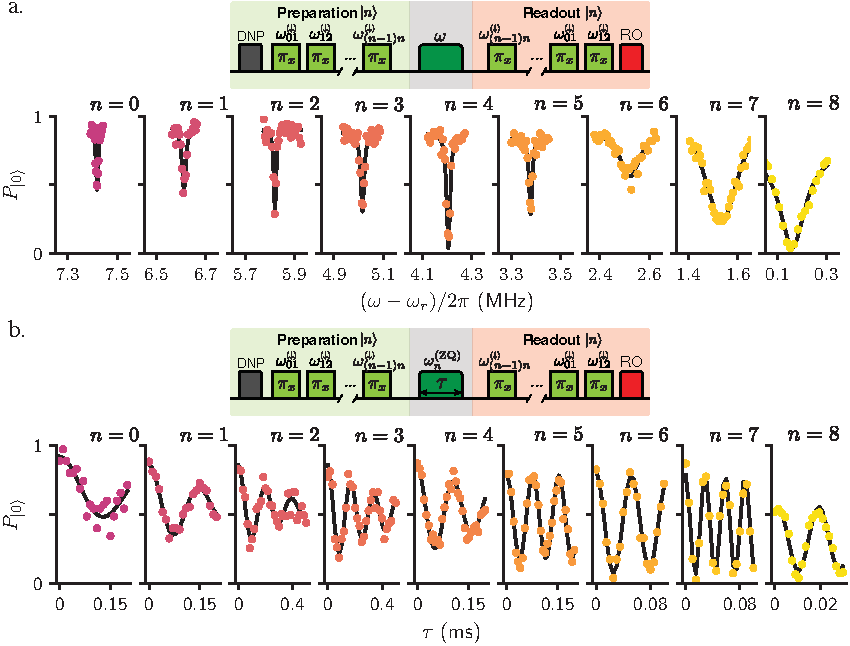
\includegraphics{chapter5/figures/zq_transitions.pdf}
    \caption[Nine ZQ transitions and Rabi oscillations]{Zero-quantum transitions and Rabi oscillations.
    \textbf{a.}
    \textit{(top)} Pulse sequence. The nuclear spin state is prepared in $\ket{n}$ A single $\pi$-pulse with frequency $\omega$ is applied on the sample and the $\ket{n}$ population is subsequently readout.
    \textit{(bottom)} Magnified view of every individual zero-quantum transition.
    \textbf{b.} 
    \textit{(top)} Pulse sequence. The pulse duration $\tau$ is swept at fixed frequency.
    \textit{(bottom)} Rabi oscillations for the zero-quantum transitions fitted to a decaying cosine oscillation (black line) for $n\in\{0,...,8\}$.}
    \labfig{zq_transitions}
\end{figure*}

\begin{marginfigure}
    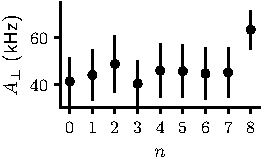
\includegraphics{chapter5/figures/A_perp_sb.pdf}
    \caption[short]{Estimated value of $A_\perp$ using the independent Rabi frequencies of the measurements in \reffig{zq_transitions}b.}
    \labfig{A_perp_sb}
\end{marginfigure}

The final pulse sequence used to polarize to state $\ket{0}$ is shown in \reffig{polarization_seq}. We sequentially drive all double-quantum transitions, starting from $n=8$ down to $n=0$, using 1~ms microwave pulses. Each pulse is followed by a 1~\textmu s delay to allow the electron spin to relax to its ground state. Because of their small matrix elements and large detuning relative to the allowed transitions, the zero- and double-quantum transitions experience large AC-Zeeman shifts, causing their resonance frequencies to be sensitive to the applied microwave amplitude. To compensate for microwave-power fluctuations and spectral drift, all pulses are chirped by 100~kHz. Due to the low Rabi rates of the sideband transitions, a single pulse is insufficient to achieve full population transfer. We therefore apply 15 repetitions of the pumping sequence to ensure reliable preparation of the \Nb nuclear spin. An additional 15 pulses are applied to the $n=0$ transition, which has the smallest matrix element and was experimentally found to be particularly difficult to polarize. Polarization into $\ket{0}$ is achieved with a probability close to $1$ at the beginning of each sequence. In addition, the $^{183}\mathrm{W}$ environment is also polarized at the beginning of every sequence to reduce the magnetic noise from the neighboring \W nuclear spins (as discussed in the next section).

\begin{figure}
    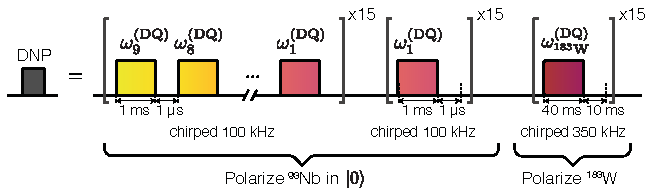
\includegraphics{chapter5/figures/polarization_seq.pdf}
    \caption[Polarization sequence]{Pulse sequence for the DNP. The sequence is separated in two distinct parts: the preparation of the \Nb spin in $\ket{0}$ and the polarization of the \W nuclear spin bath via solid effect. Pulse durations are noted as black arrows and the chirp is explicitly stated under every pulse.}
    \labfig{polarization_seq}
\end{figure}

\subsubsection{Stimulated Raman driving}

Coherent driving of the NMR transitions is performed by stimulated Raman driving at microwave frequency. Spectroscopy of the $\ket{\Downarrow,0} \leftrightarrow \ket{\Downarrow,1}$ transition is shown in \reffig{raman_spectroscopy_nb}. To measure the $\ket{\Downarrow,n} \leftrightarrow \ket{\Downarrow,n+1}$ transitions with $n>0$, we first prepare the system in $\ket{\Downarrow,n}$ by successive application of microwave Raman $\pi$ pulses from state $\ket{\Downarrow,0}$, also known as a Givens rotation \sidecite{cybenko_reducing_2001}. We then sweep the Raman detuning $\delta$. We finally measure the probability to find the system in $\ket{\Downarrow,n}$, by successive applications of $\pi$ pulses in reverse order followed by the measurement of $P_{\ket{0}}$. 

\begin{figure*}
    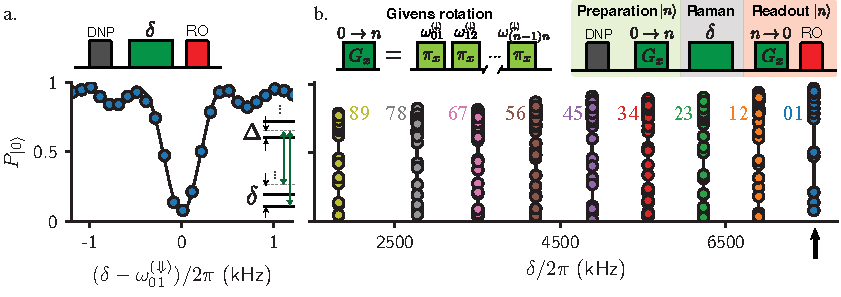
\includegraphics{chapter5/figures/raman_spectroscopy.pdf}
    \caption[NMR spectroscopy of a \Nb nuclear spin.]{
    NMR spectroscopy of a \Nb nuclear spin. 
    \textbf{a.} Raman spectroscopy for $n=0$. Population of $\ket{0}$ as a function of $\delta$. Solid black line correspond to a cardinal sine fit on the measurement data. The inset presents a diagram of the Raman driving scheme on the four-levels of interest. $\Delta$ is the detuning of one of the first pulse with the EPR transition and $\delta$ is the frequency difference between the two drives. The detuning is set to $\Delta = \omega_{01}/2$.
    \textbf{b.} \textit{(top)} Pulse sequence of spectroscopy between states $\ket{\Downarrow n}$ and $\ket{\Downarrow n+1}$. The nuclear spin is first unconditionally polarized into $\ket{0}$ followed by a Givens rotation that prepares the \Nb spin into $\ket{n}$. A Raman pulse of frequency $\delta$ is then applied. The Givens rotation is then inverted. Finally, the state of the \Nb spin is read-out. 
    \textit{(bottom)} Raman spectroscopy of all NMR transitions.  Black arrow marks the transition corresponding to the previous plot. For each transition $\Delta = \omega_{n, \ n+1}/2$.}
    \labfig{raman_spectroscopy_nb}
\end{figure*}

\begin{margintable}
\centering
\begin{tabular}{l|c}
\hline
Isotope & $\gamma / 2\pi$ (MHz/T) \\ \hline
$^{73}$Ge  & $-1.489$ \\
$^{83}$Kr  & $-1.644$ \\
$^{87}$Sr  & $-1.851$ \\
$^{93}$Nb  & $+10.452$ \\
$^{113}$In & $+9.365$ \\
$^{115}$In & $+9.386$ \\
$^{209}$Bi & $+6.962$ \\ \hline
\end{tabular}
\caption{Gyromagnetic ratios of stable nuclei with spin $I=9/2$.}
\labtab{nuclear_spin_gyromagnetic}
\end{margintable}

The spectrum of all ground state manifold NMR transitions is shown in \reffig{raman_spectroscopy_nb}b. Their frequencies span a large range, from $1.5$\,MHz to $8$\,MHz, indicating that the quadrupolar interaction has comparable magnitude to the Zeeman energy. The measured NMR frequency spectrum sheds light on the vastly different cross-relaxation lifetimes observed in \reffig{spectra_2d}b, since they scale like $\sim \omega_{n,n+1}^{2}$, explaining why low-$n$ states appear more stable.

\begin{figure}
    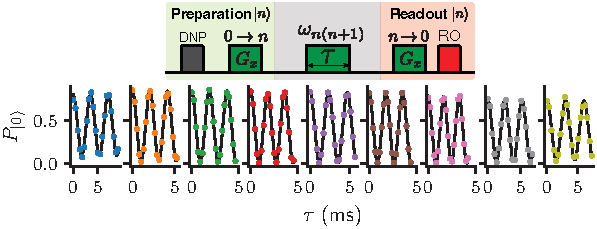
\includegraphics{chapter5/figures/raman_rabi.pdf}
    \caption[Rabi oscillations for all \Nb transitions]{Rabi oscillations for all NMR transitions. 
    \textit{(top)} Pulse sequence. We prepare state $\ket{\Downarrow n}$ followed by a resonant Raman pulse with duration $\tau$. The population of nuclear state $\ket{n+1}$ subsequently readout.
    \textit{(bottom}. Measured Rabi oscillations (colored dots) and cosine fit (solid dark line) as a function of $\tau$. The amplitude of the drives $\Omega_A$ and $\Omega_B$ was calibrated to give similar Raman Rabi frequencies.}
    \labfig{raman_rabi}
\end{figure}

\begin{marginfigure}
    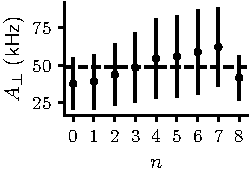
\includegraphics{chapter5/figures/A_perp_raman.pdf}
    \caption[$A_\perp$ measured through stimulated Raman driving]{$A_\perp$ measured through stimulated Raman driving. The value of $A_\perp$ measured for each transition is plot as a function of the transition index $n$. A dashed horizontal line is plot at the mean value. The error-bars show the uncertainty of the measurement obtained by error propagation, considering an uncertainty of the resonator bandwidth $\kappa$ of $50$~kHz.}
    \labfig{A_perp_sb}
\end{marginfigure}

We confirm the measurement of $A_\perp$ using the ZQ Rabi rate by estimating the value of this parameter using the stimulated Raman Rabi rate. \reffig{raman_rabi} shows the \Nb Rabi oscillations between all 9 NMR-allowed transitions fit to a cosine curve. As demonstrated in \refch{nuclea_spin_control}, the Rabi rate is proportional to $A_\perp$, and we can use Eq. \ref{eq:stimulated_raman_ninehalf_aperp} to estimate the value of this quantity. \reffig{A_perp_sb} plots the estimated $A_\perp$ as a function of $n$. The data points are centered around $A_\perp=50(11)$~kHz. The value matches quantitatively with the one measured through the sideband driving. We attribute the origin of remaining positive trend to small miss-characterization of $\omega_0$ and $\kappa$ at the time of the measurement. The resonator plays a crucial role on the filtering of the microwave amplitudes and its parameters can slowly change over time.


\section{Identification and site assignment}

The $\ket{\Downarrow,4} \leftrightarrow \ket{\Downarrow,5}$ transition frequency is particularly interesting as it is only sensitive to the quadrupolar interaction to second-order, and its frequency is therefore close to the Zeeman frequency $\omega_I + A_\parallel/2$. By comparison of $(\omega^{(\Downarrow)}_{45} - A_\parallel/2) / B_0 \simeq 10.80$~MHz/T with the tabulated values of the gyromagnetic ratio of stable nuclei with spin-9/2 (see \reftab{nuclear_spin_gyromagnetic}) we determine that the impurity is a $^{93}\mathrm{Nb}$ atom.

\begin{marginfigure}
    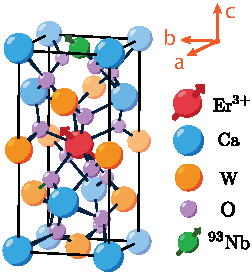
\includegraphics{chapter5/figures/crystal_with_nb.pdf}
    \caption[\Ca crystal structure with \Nb]{\Ca crystal structure with the \Er and \Nb impurities in their assigned sites.}
    \labfig{crystal_with_nb}
\end{marginfigure}

This impurity may originate from the crystal growth, or from the niobium film sputtering during resonator fabrication. We hypothesize that the niobium atom enters in substitution of a $\mathrm{W}^{6+}$ atom in a pentavalent state, thus compensating the \Er extra positive charge compared to $\mathrm{Ca}^{2+}$. From $A_\parallel/2\pi \sim 130$\,kHz (see \reffig{spectra_2d}b), and $A_\perp/2\pi \sim 50$\,kHz, we determine that the \Nb is located 0.5\,nm from the \Er along the $c$ axis, as shown in \reffig{crystal_with_nb}. We confirm this assignment by measuring $A_\parallel$ and $A_\perp$ for various in-plane angles $\theta$.

\reffig{site_assignment}a plots the measured values of $A_\parallel$ and $A_\perp$ along with the numerical estimations for all 10 possible W positions in the first unit cell. The numerical estimations quantitatively agree with the measured coupling for the assigned site with the coupling for a type 3 position, which lies directly along the $c$-axis. Figure \reffig{site_assignment}b shows a magnified version of the plot. We note a systematic shift for the values of $A_\parallel$ of less than 1\% with respect to the measured values, which may be due a breakdown of the point-dipole approximation, or to a slight shift of the \Nb position with respect to the \W site, possibly also impacted by strain caused by differential thermal contraction of the \Nb thin-film and the \Ca substrate \cite{pla_straininduced_2018,billaud_electron_2025}. 

\begin{figure*}
    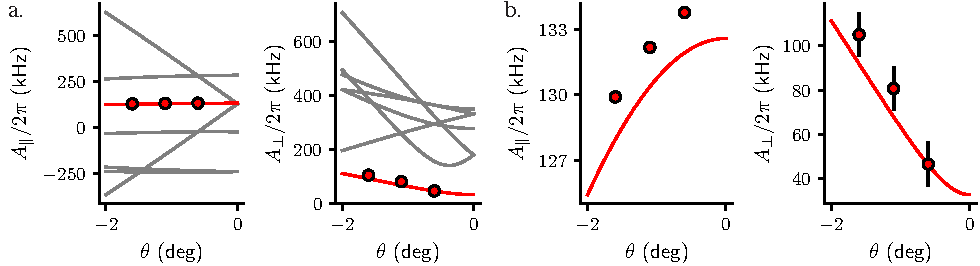
\includegraphics{chapter5/figures/site_assignment.pdf}
    \caption[Measured and calculated hyperfine coupling as a function of $\theta$]{Measured and calculated hyperfine coupling as a function of $\theta$.
    \textbf{a.} Calculated hyperfine couplings $A_{\parallel}$ and $A_{\perp}$ (left and right panels, respectively) as a function of the in-plane angle $\theta$ between \Er and \Nb for all ten neighboring W sites in the first unit cell (colored lines), together with the experimentally measured values (black points). The numerical estimates take into consideration the misalignment angle $\beta_0$ between the resonator plane and the crystal $c$-axis.
    \textbf{b.} Magnified view of the relevant region only showing the coupling for the assigned site. Error-bars for the $A_\parallel$ measurement are plot, but hidden by the marker.
    }
    \labfig{site_assignment}
\end{figure*}


\section{Precision NMR spectroscopy}

\begin{figure*}
    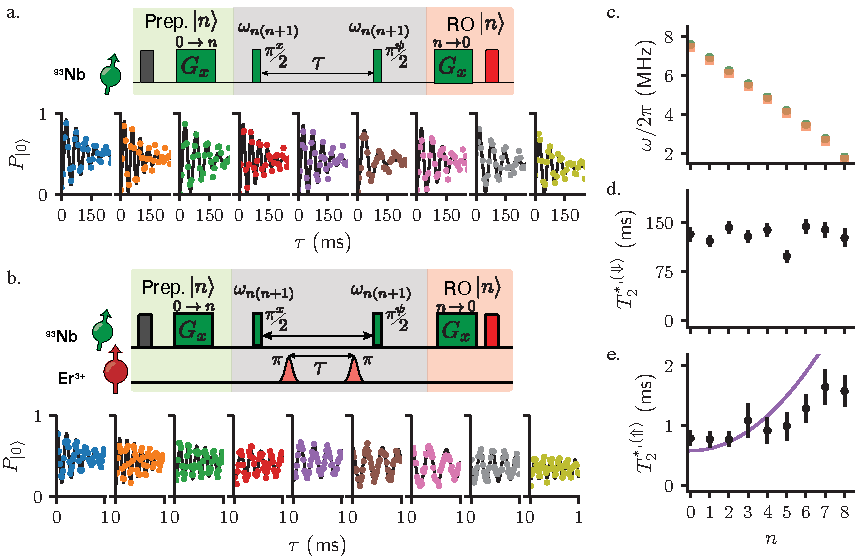
\includegraphics{chapter5/figures/ramsey_ninehalf.pdf}
    \caption[\Nb Ramsey measurements]{Ramsey measurements of the \Nb transitions. 
    \textbf{a.} \textit{(top)} Ramsey, pulse sequence between states $\ket{\Downarrow n-1}$ and $\ket{\Downarrow n}$. 
    \textit{(bottom)} Population of $\ket{0}$ as a function of $\tau$ for $n=0$. Solid black line corresponds to a cosine fit with a decaying exponential.
    \textbf{b.} \textit{(top)} Excited Ramsey pulse sequence.
    \textit{(left)} Population of $\ket{0}$ as a function of $\tau$ for $n=1$. Solid black line corresponds to a cosine fit with a decaying exponential.
    \textbf{c.} \Nb nuclear spin transition frequency $\omega^{(\Downarrow)}_{n, \ n+1}$ and $\omega^{(\Uparrow)}_{n, \ n+1}$ (green and blue markers resp.) as a function of $n$. 
    \textbf{d.} Coherence $T_2^{*, (\Downarrow)}$ for each transition $\ket{\Downarrow n}\leftrightarrow\ket{\Downarrow, n+1}$.    
    \textbf{e.}  Coherence $T_2^{*, (\Uparrow)}$ for each transition $\ket{\Uparrow n}\leftrightarrow\ket{\Uparrow, n+1}$. Solid line gives an upper bound to the coherence from the relaxation rate through the Purcell effect. 
    Error bars in the figures correspond to the 1-$\sigma$ fit uncertainty.}
    \labfig{ramsey_ninehalf}
\end{figure*}

The accuracy of the NMR spectra measured in \red{sec} is reduced due to the differential AC-Zeeman shifts, that renormalize the energy levels of the system under the stimulated Raman pulses. A straightforward way to increase both the accuracy and the precision of the measurement is to leverage the long coherence time of the nuclear spins through a Ramsey sequence. Indeed, the frequency of the oscillations in a Ramsey measurement directly map to the bare frequency difference between the two levels of interest, provided that no pulse is applied during the free-evolution time of the sequence. 

\subsubsection{Ramsey measurements}

We first measure the ground-state-manifold frequencies $\omega^\Downarrow_{n,n+1}$. We prepare the system in $\ket{\Downarrow,n}$, apply two Raman $\pi/2$-pulses on the $\ket{\Downarrow,n} \leftrightarrow \ket{\Downarrow,n+1}$ transition separated by a time $\tau$, and measure the resulting probability to find the \Nb in $\ket{n}$. The phase of the second $\pi$-pulse has an artificial detuning to compensate for the rapid natural oscillations of the population. The data for all transitions is shown in \reffig{ramsey_ninehalf}a, together with an exponential cosine fit. 

The excited-state manifold frequencies $\omega^\Uparrow_{n,n+1}$ are then measured by including two \Er $\pi$-pulses separated by $\tau$, applied in-between two Raman $\pi/2$ pulses kept at a constant time delay of $1$\,ms. The oscillation frequency directly yields $\omega^\Downarrow_{n,n+1}-\omega^\Uparrow_{n,n+1}$ (see \reffig{ramsey_ninehalf}b). 

\reffig{ramsey_ninehalf}c plots the fitted NMR frequencies as a function of the transition index $n$, both for the ground and excited state of the \Er spin (green and blue resp.). The ground state transitions and consistently larger than their excited state counterparts, which indicate a positive value of $A_\parallel\approx130$~kHz. 

The fitted coherence time for ground and excited Ramseys are in plot in \reffig{ramsey_ninehalf}d and e respectively. The ground state transitions display a constant behavior with $T_2^*\approx150$~ms.\sidenote{We note that for $n=5$ the coherence time is slightly lower for unknown reasons.}. This indicates that magnetic noise is the dominant contribution to the Ramsey dephasing, since electric noise would impact more strongly transitions with extremal values of $n$, as was observed in an individual $^{123}\mathrm{Sb}$ nuclear spin in silicon \sidecite{fernandezdefuentes_navigating_2024}. As expected, the coherence time of the excited state Ramsey measurements is limited by the \Er relaxation time. We observe that $T_2^{*(\Uparrow)}$ slightly increases with $n$, due to the increased detuning of the $\ket{\Downarrow,n} \leftrightarrow \ket{\Uparrow,n}$ transition from the resonator. The increase is less than expected from the Purcell effect, shown as a purple line in the plot, suggesting that this \Er has a relatively short non-radiative lifetime, of order $\sim 3$\,ms, possibly linked to the proximal \Nb impurity. 

\begin{marginfigure}
    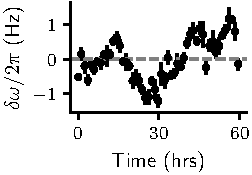
\includegraphics{chapter5/figures/drift.pdf}
    \caption[\Nb transition frequency drift]{Frequency drift of the $\ket{\Downarrow 0} \leftrightarrow \ket{\Downarrow 1}$ transition as a function of time. Dashed line highlights $\delta \omega = 0$. Error-bars correspond to the 1-$\sigma$ uncertainty of the fitted Ramsey measurement.}
    \labfig{drift}
\end{marginfigure}

From the fitted coherence we estimate that the uncertainty of the measured frequencies is approximately $\sim 1$~Hz for the ground state and $\sim 20$~Hz for the excited state. We confirm this conclusion by monitoring the frequency drift of the $\ket{\Downarrow 0} \leftrightarrow \ket{\Downarrow 1}$ transition during a prolonged period of 60 hours. \reffig{drift} plots the frequency drift $\delta \omega$ as a function of time, which remains confined within $\pm1$~Hz.

\subsubsection{The effect of the \W bath}

The nuclear spin bath, consisting of neighboring \W\ nuclear spins, significantly contributes to the spectral drift of the \Nb\ transition frequencies. To mitigate this effect, we polarize the spin bath using solid-effect DNP by applying microwave pulses resonant with the double-quantum transitions of the coupled \W\ spins. To be able to effectively drive weakly coupled \W nuclear spins, we employ 40~ms pulses separated by 10~ms delays to allow the microwave lines to cool, and repeat this sequence 15 times. The strong pulse amplitudes induce a substantial AC-Zeeman shift, and we account for this by chirping the pulse 350~kHz around $\omega^{\mathrm{(W)}}/2\pi = 725$~kHz. Note that it is crucial that the \W\ polarization sequence is applied \emph{after} the \Nb\ preparation, since the electron-spin allowed transition depends on the \Nb\ state, and the \W\ double-quantum transition is correspondingly detuned relative to this transition.

\begin{figure}
    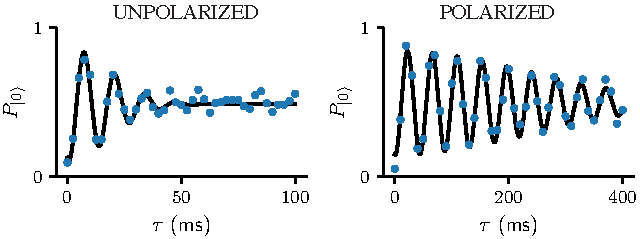
\includegraphics{chapter5/figures/polarized_vs_unpolarized.pdf}
    \caption[Effect of \W polarization]{Ramsey sequence with and without \W polarization pulses. Measurement data (dots) are fit to an exponentially decaying (line) which yields $T_2^*=22$~ms and $T_2^*=331$~ms for the unpolarized and the polarized case respectively.}
    \labfig{polarized_vs_unpolarized}
\end{figure}

To demonstrate the impact of the \W polarization, \reffig{polarized_vs_unpolarized} shows a \Nb Ramsey measurement with and without \W polarization. The \Nb coherence time $T_2^*$ without \W polarization is $26$\,ms, and it increases up to 331~ms upon polarizing the \W bath.

\subsubsection{Hahn echo measurements}

In addition, the large nuclear spin of \Nb offers interesting perspectives for quantum sensing. Indeed, the magnetic moment of states $0$ and $n$ differ by $\sim n \, \mu_\text{\Nb}$, implying that the state $\ket{0} + \ket{n}$ is $\sim n$ times more sensitive to a small magnetic signal than $\ket{0} + \ket{1}$. Such "Schrödinger spin-cat" states have been studied in a Sb donor in silicon~\sidecite{yu_creation_2024}, and used in magnetometry with Rydberg atoms sensing \sidecite{dietsche_highsensitivity_2019}. We perform a preliminary characterization of the magnetic sensitivity of these states by measuring the echo coherence of the state $\ket{\Downarrow \, 0} + \ket{\Downarrow \, n+1}$. Figure \reffig{echo_nb}a \& b show a schematic of the pulse sequence along with the signal, fitted to an exponentially decaying cosine which yield the coherence time $T_{2}$. The decoherence rate $1/T_2$ is seen to increase linearly with $n$ (see \reffig{echo_nb}c), indicating that decoherence occurs mainly because of magnetic noise. Due to the accumulation of coherent errors on the pulses, we only measure these states until $n=$. These measurements were taken in a different magnetic field configuration with a misalignment angle $\theta=-0.3^\circ$. 

\begin{figure*}
    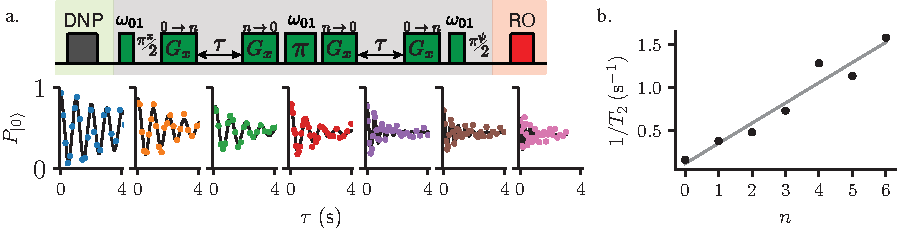
\includegraphics{chapter5/figures/echo.pdf}
    \caption[Hahn echo coherence]{Hahn echo for all $\ket{\Downarrow 0}$ and $\ket{\Downarrow n}$ pairs.
    \textbf{a.} Pulse sequence. 
    \textbf{b.} Measurement data (dots) is plot alongside an exponentially decaying fit (black solid lines). 
    \textbf{c.} Decoherence rate $1/T_2$ for all $\ket{\Downarrow 0}$ and $\ket{\Downarrow n}$ pairs. Measurements (dots) are fit to a linear trend (black line).}
    \labfig{echo_nb}
\end{figure*}


\section{Hamiltonian fit}

\subsection{Fitting $\mathcal{H}^{(\Downarrow)}$ and $\mathcal{H}^{(\Uparrow)}$}

We now analyze the frequency data shown in \reffig{ramsey_ninehalf}c to extract the nuclear spin parameters.  We first fit the frequencies in the \Er ground and the excited state using $\mathcal{H}^{(\Downarrow)}$ and $\mathcal{H}^{(\Uparrow)}$, respectively (Eq. \ref{eq:up_down_hamiltonian}). These fits are independent and can be effectively understood as describing a nuclear spin experiencing different effective magnetic fields in the two states, differing in both magnitude and orientation due to the parallel and perpendicular components of the hyperfine interaction. Before proceeding to the fit, we note an intrinsic degeneracy of the quadrupole spectrum when only measured along a single magnetic field orientation.

\subsubsection{Rotational invariance of the quadrupolar energy spectrum}

When fitting the nuclear transition frequencies in this work, we consider the measurements with a single orientation of the magnetic field. Under these conditions, the measured NMR frequencies are not sufficient to describe the full quadrupole tensor. It is intuitively clear that the measured spectrum should be invariant under a rotation around the applied field direction $z$, and that therefore only parameters $4$ can be determined at best. This is clearly evidenced when expressing the quadrupole tensor as a function of rank-2 spherical tensors $T^{(2)}_{m}$, instead of Cartesian coordinates. \sidenote{
The rank-2 spherical tensors are related to the spin operator basis by
\begin{equation*}
\begin{split}
T^{(2)}_{0} &= 3 I_z^2 - I(I+1), \\
T^{(2)}_{\pm 1} &= \mp \left( I_z I_{\pm} + I_{\pm} I_z \right), \\
T^{(2)}_{\pm 2} &= I_{\pm}^2 .
\end{split}
\end{equation*}
}. By algebraic manipulation we can rewrite the quadrupolar interaction as

\begin{equation}
    \cH{Q} / \hbar = \mathbf{I} \cdot \bar{\bar{Q}} \cdot \mathbf{I} = \sum_{m = -2}^2 Q_m T^{(2)}_m(\hat{\mathbf{I}})
    \label{eq:quadrupole_spherical}
\end{equation}

\noindent with

\begin{equation}
\begin{aligned}
Q_{0} &= Q_{zz}, \\
Q_{\pm 1} &= Q_{zx} \pm i Q_{zy}, \\
Q_{\pm 2} &= \tfrac{1}{2}(Q_{xx} - Q_{yy}) \pm i Q_{xy}.
\end{aligned}
\end{equation}

One can show (Appendix \ref{app:rotations_quadrupole}) that the coefficients transform as 
\begin{equation}
Q_m \;\mapsto\; e^{-im\zeta}\, Q_m,
\end{equation}
under a physical rotation of angle $\zeta$ about the $z$-axis. Since the energy levels of the Hamiltonian are insensitive to these phase factors and depend only on invariants such as $Q_0$, $|Q_{\pm 1}|^2$, and $|Q_{\pm 2}|^2$, the energy spectrum is invariant under such rotations. The matrix form of the quadrupole tensor in terms of these invariants is

\begin{align}
\begin{split}
    \bar{\bar{Q}}(\zeta) =&\begin{pmatrix}
-|S_2| \cos(2\zeta+2\Delta)-\frac{S_0}{2}&  |S_2|\sin(2\zeta+2\Delta) & |S_1|\cos(\zeta) \\ 
|S_2| \sin(2\zeta+2\Delta)  & |S_2|\cos(2\zeta+2\Delta)-\frac{S_0}{2} & |S_1|\sin(\zeta) \\
|S_1|\cos(\zeta) & |S_1|\sin(\zeta) & S_0\end{pmatrix} \\\\
\end{split}
\end{align}

where $\Delta$ is the phase difference between $S_{+2}$ and $S_{+1}$

\begin{equation}
\Delta = \Delta_2 - \Delta_1 = \arctan\left(\frac{2Q_{xy}}{Q_{xx}-Q_{yy}}\right) -  \arctan\left(\frac{Q_{yz}}{Q_{xz}}\right)
\end{equation}

For single axis measurements, this leaves $S_0$, $|S_1|$, $|S_2|$, and $\Delta$ to be determined, whereas $\zeta$ can be fixed to an arbitrary value. This is a subtle point with an important consequence: any two tensors related by a rotation in the $xy$ plane produce identical NMR spectra for a fixed field orientation\sidenote{It is straightforward to see that the Zeeman term is also degenerate under rotations along the axis of $B_0$.}. Equivalently, no matter how precise the measurement of the nuclear transition frequencies, one can only reconstruct the quadrupole tensor up to a rotation about the field axis. Consequently, the only way to lift this degeneracy is by measuring with a different quantization axis of the nuclear spin\sidenote{At zero magnetic field, no orientation information can be extracted, only the magnitudes of the principal components of the quadrupole}.

\subsubsection{Monte Carlo Markov Chains}

We now focus on fitting the ground state Hamiltonian $\mathcal{H}^{(\Downarrow)}$ to the measured data, but the procedure is identical for $\mathcal{H}^{(\Uparrow)}$. We recall that 

\begin{equation}
    \mathcal{H}^{(\Downarrow)}/\hbar = -\omega_S / 2 + \omega_I^{(\Downarrow)} I_z^{(\Downarrow)} + \mathbf{I^{(\Downarrow)}}\cdot \bar{\bar{Q}}^{(\Downarrow)}\cdot \mathbf{I^{(\Downarrow)}}.
\end{equation}

The parameters to fit are $B^{(\Downarrow)}_0 = - \omega_I^{(\Downarrow)} / \gamma_\text{\Nb}$ and $\bar{\bar{Q}}^{(\Downarrow)}$, where $B^{(\Downarrow)}_0$ is the effective magnetic field the \Nb spin observes when the \Er is in the ground state, which combines the external field $B_0$ and the effective field generated by the \Er spin. When parameterizing the quadrupole in terms of the rank-2 spherical tensors, the total set of variables to fit is defined as $\mathcal{V^{(\Downarrow)}} \equiv\{B^{(\Downarrow)}_0, S^{(\Downarrow)}_0, S^{(\Downarrow)}_1, S^{(\Downarrow)}_2, \Delta^{(\Downarrow)}\}$ and $\zeta$ is arbitrarily set to 0. We note that another degeneracy inherent to the one-axis nature of the measurement is the sign of $S_1^{(\Downarrow)}$ and $S_2^{(\Downarrow)}$ as well as $\Delta^{(\Downarrow)}$, that is periodic between $-\pi/4$ and $\pi/4$. For the purposes of the fit, we set the following priors

\begin{equation}
    S_1^{(\Downarrow)} > 0 \quad | \quad S_2^{(\Downarrow)}>0 \quad | \quad -\pi/4 <\Delta^{(\Downarrow)} < \pi/4
\end{equation}

The ground state NMR transitions $\omega_{n,\ n+1}^{\text{fit}}(\mathcal{V^{(\Downarrow)}})$ are calculated by numerically diagonalizing $H^{(\Downarrow)}(\mathcal{V}^{(\Downarrow)})$ and taking the energy differences between the relevant energy levels. We define the following likelihood

\begin{equation}
    \mathcal{L}^{(\Downarrow)}(\mathcal{V}^{(\Downarrow)}) = \sum_{n=0}^9 \left(\frac{\omega^{(\Downarrow)}_{n, \ n+1} - \omega_{n, \ n+1}^{\text{fit}}(\mathcal{V^{(\Downarrow)}})}{\sigma^{(\Downarrow)}_{n, \ n+1}}\right)^2,
\end{equation}

where $\sigma^{(\Downarrow)}_n=1$~Hz is the measurement uncertainty. The Hamiltonian fit was performed via Monte-Carlo Markov-Chain simulation \cite{foreman-mackey_emcee_2013}. In brief, the algorithm initializes an arbitrary number of walkers, or particles, in the parameter space. After an evaluation of the logarithm of the likelihood function, the positions of the walkers are updated through the "stretch move" \cite{goodman_ensemble_2010} with the objective of minimizing the evaluation for the next iteration. We run the algorithm with 64 walkers and 60000 iterations, from which we obtain the following median values for the ground and excited state parameters

\begin{align}
\begin{split}
    &B^{(\Downarrow)}_0 =  460.8320(4)\text{~mT} \; | \; S^{(\Downarrow)}_0 = -237.3609(6)\text{~kHz}\\  
    S^{(\Downarrow)}_1& = 2.08(5) \text{~kHz} \; | \;  S^{(\Downarrow)}_2 = 149.456(6)\text{~kHz}\; | \; \Delta^{(\Downarrow)} = 0.2(1) \\ 
    \\
    &B^{(\Uparrow)}_0 = 447.994(6)\text{~mT} \; | \; S^{(\Uparrow)}_0 = -237.256(9)\text{~kHz} \\
    S^{(\Uparrow)}_1& = 5.0(3)\text{~kHz} \; | \; S^{(\Uparrow)}_2 = 149.48(8)\text{~kHz}\; | \; \Delta^{(\Uparrow)} = 0.2(1)
\end{split}
\end{align}

\begin{figure}
    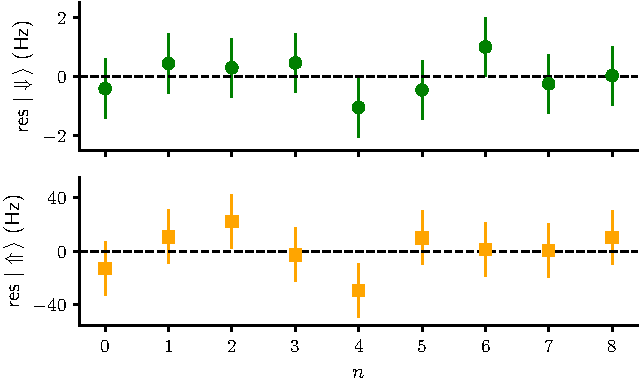
\includegraphics{chapter5/figures/fit_residuals.pdf}
    \caption[Residuals for the $\mathcal{H}^{(\Downarrow)}$ and $\mathcal{H}^{(\Uparrow)}$ fit]{Residuals for the $\mathcal{H}^{(\Downarrow)}$ and $\mathcal{H}^{(\Uparrow)}$ fit, top and bottom respectively. Error-bars correspond to the uncertainty of the measured values. Dashed line corresponds to zero deviation.}
    \labfig{fit_residuals}
\end{figure}

The residuals of the two fits are shown in \reffig{fit_residuals}. The results agree up to statistical uncertainty ($1$\,Hz for the $\Downarrow$ data, $20$\,Hz for the $\Uparrow$ data), and the residuals show no discernible trend.  We calculate the reduced chi-squared for the ground and excited state and obtain $\chi^{2,(\Downarrow)}_\nu=0.75$ and $\chi^{2,(\Uparrow)}_\nu=1.14$, respectively. The proximity of these values to 1 indicates that the model correctly describes the data while avoiding over-fitting. We remark that the uncertainty of $S_1^{(\Downarrow)}$ and $\Delta^{(\Downarrow)}$ is much larger than the other parameters. This is readily explained by the effect of these quantities on the energy levels of the Hamiltonian. On the one hand, $S_1$, $\Delta$ are closely related to the values of the quadrupole perpendicular to $B_0$, and are only observable as second and third order effects respectively. On the other hand, $B_0$, $S_0$ and $S_2$ are responsible for zero and first order effects and their estimation is more precise. 

The fit returns the quadrupolar tensors $\bar{\bar{Q}}^{(\Downarrow)}$ and $\bar{\bar{Q}}^{(\Uparrow)}$, up to an arbitrary rotation around the $z^{(\Downarrow)}$ and $z^{(\Uparrow)}$ axes, respectively. We compare the principal values of the tensor obtained via diagonalization\sidenote{The tensors are expressed in different Cartesian bases, determined by the nuclear spin quantization axis in each manifold, which means that direct component-wise comparison is inappropriate}. This analysis reveals that the principal axis associated with the largest eigenvalue (denoted $X$) lies approximately within the crystal $(a,b)$-plane, up to an undetermined in-plane angle. The second-strongest principal axis (denoted as $Z$) is approximately parallel to the crystal $c$-axis and therefore to $B_0$. 

\begin{figure}
    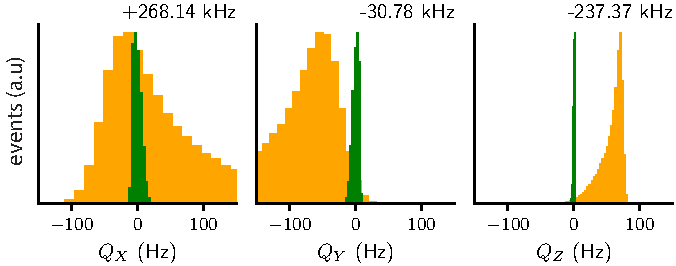
\includegraphics{chapter5/figures/q_histograms.pdf}
    \caption[Quadrupole principal values]{Posterior distribution of the quadrupole tensor principal components for $\mathcal{H}^{(\Downarrow)}$ and $\mathcal{H}^{(\Uparrow)}$ (green and orange resp.). The distributions are normalized to the same height for visual clarity.}
    \labfig{q_histograms}
\end{figure}

\red{should we show the full set of posterior distributions?}

The posterior distribution of the quadrupole principal values are shown in \reffig{q_histograms} for both \Er spin states. The main result is the existence of a statistically-significant ($3\sigma$) difference between the values of $Q_{Z}^{(\Uparrow)}$ and $Q_{Z}^{(\Downarrow)}$. Due to the larger uncertainty on $Q_{X}$ and $Q_{Y}$, this observation is not reproduced on $X$ or $Y$. Consequently, our results indicate the existence of a new term in the spin Hamiltonian Eq.~\ref{eq:hamiltonian_ninehalf_full}, which modifies the nuclear quadrupolar interaction depending on the electron spin state. 

\subsection{Fitting $\mathcal{H}$}

To further test our model, we take a step back in the approximations and fit the complete frequency dataset. In addition, we now introduce a term that models the electron spin dependent nuclear quadrupole. Given that our measurements are maximally sensitive along the $z$ axis, we approximate this term in analogy to a standard quadrupole term, 

\begin{equation}\label{eq:SDQ}
\mathcal{H}_\mathrm{sdq} = \frac{C_\mathrm{sdq}}{4 I (2I-1)} S_z \left(3 I_z^2 - I(I+1) \right).
\end{equation}

Where $C_\mathrm{sdq}$ is the interaction coupling strength. Moreover, to account for the high spectral resolution of our data we include in the Hamiltonian higher order terms we have previously disregarded. 

%First, we consider non-secular hyperfine terms, which are estimated by magnetic dipole interaction simulations (see \red{ref}) and are fixed during the fitting procedure. 

\subsubsection{Lamb shift}

First, we consider the Lamb shift of the electron spin transitions, which renormalize the \Nb transitions in the excited state of the \Er spin. As discussed in \red{sec}, the Lamb shift of the excited state of a spin-1/2 coupled to a resonator in its (vacuum) ground state, with coupling strength $g_0$ and detuning $\Delta$ is given by

\begin{equation}
\Delta\omega = \Delta \frac{g_0^2}{\Delta^2 + \kappa^2/4}.
\end{equation}

In the case of the coupled \Nb--\Er system, the \Er excited state levels $\ket{\uparrow,n}$ are shifted by $\Delta \omega_n = g_0^2 \frac{\Delta_n}{\Delta_n^2 + \kappa^2/4}$, where $\Delta_n = \omega_0 - \omega_n$ is the detuning of the EPR-allowed transition from the resonator frequency. The order of magnitude is $\Delta \omega \sim g_0^2 / \kappa \sim 2\pi \times 100\,\mathrm{rad}\cdot \mathrm{s}^{-1}$ and the dependence on $n$ causes shifts $\Delta_{n+1} - \Delta_n$ of the NMR transition frequencies $\omega_{n,n+1}^\Uparrow $, which therefore must be taken into account in our analysis. 

This is achieved by adding a term

\begin{equation}
    \mathcal{H}_L = \Delta \omega_n \ket{\Uparrow,n}\bra{\Uparrow,n}
\end{equation}

\subsubsection{Non-secular hyperfine}

Second we consider non-secular hyperfine terms, which are estimated by magnetic dipole interaction simulations (see \red{ref}) and are fixed during the fitting procedure. Additionally, we fix the perpendicular hyperfine term to the measured value in \red{sec} $A_\perp = 46$~kHz to effectively reduce the number of variables to fit.


\subsubsection{Final Hamiltonian}

Combining all the terms, the full Hamiltonian of an \Er:\Ca spin coupled to a \Nb nuclear spin (and to its detection resonator) is

\begin{align}
\begin{split}
        \mathcal{H}/\hbar &= \omega_S\cdot S_z + \omega_I\cdot I_z +\mathbf{S} \cdot \bar{\bar{A}} \cdot \mathbf{I} + \mathbf{I} \cdot \bar{\bar{Q}} \cdot \mathbf{I} + \\ 
        &+ \frac{C_\mathrm{sdq}}{4 I (2I-1)} S_z [3 I_z^2 - I(I+1) ]  + \Delta \omega_n \ket{\uparrow,n}\bra{\uparrow,n}
\end{split}
\end{align}

Note that because the Hamiltonian is not invariant by rotation around the $z$ axis, the full quadrupolar tensor can now be obtained. Following the parameterization presented in \red{ref}, the set of eight variables to fit is defined as $\mathcal{V}\equiv\{B_0, A_\parallel, S_0,S_1,S_2,\Delta,\zeta,Q^{\text{(SDQ)}}_{zzz}\}$. Naturally, we define the total likelihood as

\begin{equation}
    \mathcal{L}(\mathcal{V}) = \mathcal{L}^{(\downarrow)}(\mathcal{V}) + \mathcal{L}^{(\uparrow)}(\mathcal{V}).
\end{equation}

The fit is performed by repeating the MCMC algorithm described in the previous section for 400 different values of $A_\perp$, sampled from a Gaussian distribution with a standard deviation of 9~kHz. The median values for the parameters, obtained from the resulting ensemble of fits, are given by

\begin{align}
\label{seq:full_fit_results}
\begin{split}
    B_0 =  454.408(3)\text{~mT} \; &| \; A_\parallel =  133.751(5)\text{~kHz} \\ 
    S_0 = -237.314(3)\text{~kHz} \; &| \; S_1 = -3.44(1) \text{~kHz} \\
    S_2 = -149.457(5)\text{~kHz}\; &| \;  \red{Q_{zzz}^{(SDQ)} = 76(4)} \text{~Hz}\\
    \Delta = 1.62(2)\; &| \;\zeta = 0.9(1), \\
\end{split}
\end{align}

\noindent with a reduced chi-squared of $\chi^2_\nu=1.2$, with similar residuals as the ones reported in \reffig{fit_residuals}. 

From these values, we reconstruct the nuclear quadrupole tensor $\bar{\bar{Q}}$ and diagonalize it to obtain its principal axes $X$, $Y$, and $Z$. We find that the $Z$ axis is tilted by $0.06(3)^\circ$ with respect to the crystal $c$ axis, while the $X$ axis is rotated by $-10(6)^\circ$ relative to the crystal $a$ axis. The corresponding principal values are $Q_X = 268.138(9)$~kHz, $Q_Y = -30.799(7)$~kHz, and $Q_Z = -237.338(3)$~kHz. These values correspond to a quadrupolar interaction strength of $C_q / 2\pi = 19.3059(7)\,\mathrm{MHz}$ and a biaxiality parameter $\eta = 0.77026(7)$.

The quadrupolar tensor $\bar{\bar{Q}}$ is graphically represented in the crystal frame in \red{fig}. We compare the fitted quadrupole tensor with DFT calculations performed by our theory collaborator Thibault Charpentier. The simulations yield $C_{q,\text{DFT}}=22.7$~MHz, $\eta_{\text{DFT}}=0.76$, and similar orientation of the principal axes, in close agreement with the fitted values. This confirms that $\mathrm{Nb}^{5+}$ replaces $\mathrm{W}^{6+}$. Finally, the SDQ term \red{$Q^{(\text{SDQ})}_{zzz}/2\pi= 76(4)$~Hz} is fitted to a non-zero value with a high degree of confidence. We check the consistency and reproducibility of our analysis by repeating these measurements for a small range of in-plane angles $\theta$ (see \red{fig}). Despite the vastly different values of the Hamiltonian parameters (in particular, $\omega_I$ and $A$), the values extracted for \red{$Q^\text{(SDQ)}_{zzz}$} remain approximately unchanged. 